\documentclass[9pt,technote]{IEEEtran}

\usepackage{mathtools}
\usepackage{tipa}
\usepackage{amsmath}
\usepackage{algorithmic}
\usepackage{array}
\usepackage{subfigure}
\usepackage{pgf}
\usepackage{lmodern}
\usepackage[justification=centering,font=footnotesize,labelfont=bf]{caption}
\usepackage{flushend}
\usepackage{lipsum}
\usepackage{braket}
\usepackage{xcolor}
\usepackage{float}
\usepackage{booktabs}
\usepackage{graphicx}
\usepackage{stfloats}
\usepackage{quantikz}

\usepackage{tikz}
\usetikzlibrary{fit,shapes,positioning,calc,shapes.geometric,backgrounds,quantikz2}

\colorlet{tempGray}{gray!80!cyan}
\colorlet{lightgray}{tempGray!60!white}
\colorlet{orange}{red!30!yellow}
\colorlet{lightorange}{orange!60!white}
\definecolor{purple}{RGB}{207,81,212}

% --- Wavelength colours for WDM ---
\definecolor{wl1}{RGB}{220, 50,  50}   % red    λ₁
\definecolor{wl2}{RGB}{200, 140, 0}    % amber  λ₄
\definecolor{wl3}{RGB}{50,  160, 50}   % green  λ₂
\definecolor{wl4}{RGB}{50,  80,  220}  % blue   λ₃
\definecolor{fibreclr}{RGB}{200, 220, 240}
\definecolor{boxclr}{RGB}{240, 245, 255}

\tikzset{
  comp/.style  = {draw, rounded corners=4pt, fill=boxclr,
                  minimum width=2.0cm, minimum height=3.8cm,
                  align=center, font=\small\bfseries},
  fibre/.style = {draw, fill=fibreclr, minimum width=4.5cm,
                  minimum height=1.2cm, rounded corners=2pt},
  arr/.style   = {-{Stealth[length=4pt]}, line width=1.2pt},
  lbl/.style   = {font=\footnotesize},
}


\hyphenation{op-tical net-works semi-conduc-tor}
\usepackage[hyphens]{url}
\usepackage{hyperref}


\begin{document}

\title{From Lab to Field: A Comparison of Implementation and Deployment of MDI-QKD and BB84}

\author{Linus~Kelsey%
\thanks{Submitted for the Literature Review (portion of the Research Project) toward the award of MSc Quantum Technologies at University College London.}%
\thanks{\textit{Email}: alfred.kelsey.25@ucl.ac.uk}%
\thanks{Supervised by Dr. Alejandra Beghelli and Dr. Emilio Hugues Salas, both of BT Group.}%
\thanks{Manuscript compiled \today.}}


% The paper headers
\markboth{UCL MSc Quantum Technologies -- Literature Review}%
{Kelsey: On MDI-QKD}

% make the title area
\maketitle

\begin{abstract}
Quantum Key Distribution (QKD) was first proposed in 1984 by Bennett and Brassard through their foundational Prepare-and-Measure (PM) QKD protocol, commonly known as BB84, as a class of secure key exchange routines. In the following decades, a number of novel processes have emerged as alternative methods of exploiting quantum physics to guarantee shared secrecy. In particular, Measurement-Device-Independent (MDI) QKD was presented in 2012, providing improved security assumptions over BB84 by removing the need to trust qubit detectors. We present a review of the literature surrounding physical realisations of and platforms for the hosting of MDI QKD links and networks, with comparison to BB84 provided, motivating a parametric simulation-based comparison of the two protocols in the companion report.
\end{abstract}

\begin{IEEEkeywords}
Quantum Key Distribution, Device-Independence, Platforms \& Hosting
\end{IEEEkeywords}


\section{Introduction}

The advent of Quantum Computing promises to bring with it the promise of great changes to our technological infrastructure. Cybersecurity finds itself at risk, as novel computation brings novel digital threats. Modern encryption key exchange standards, including RSA \cite{RSA_1978} and Elliptic Curve Cryptography (\cite{Koblitz_ECC} and \cite{Miller_ECC}, independently) hinge on the difficulty for classical computers to compute integer factorisations. Shor's algorithm \cite{Shor_1997}, presented first in 1995 and published two years later, demonstrated a period-finding quantum algorithm to factor integers in polynomial time. This presented an exponential speed-up over the best known classical methods (to this day), and therefore an efficient route to decrypt factorisation-based standards. Key sharing protocols based on the Discrete Log Problem, like Diffie-Helman \cite{DiffieHellman}, are also beaten by a variant of Shor's work. To move past this looming vulnerability we must determine cryptographic primitives which are resistant to quantum advantage. Classical methods with security imposed by problems not sped up by quantum computers are known as Post-Quantum Cryptography (PQC), while others have sought to use quantum to the benefit of the encrypting parties.

QKD is one such way - proposed, initially, by Stephen Wiesner \cite{Wiesner_1983} in the 1970's (though his work was not published until 1983). This was soon followed by Bennett and Brassard's revolutionary paper \cite{Bennett_2014} providing a method by which to establish shared secrecy through quantum methods. In the decades since, QKD has developed into one of the most field-tested quantum technologies, with national-scale deployments \cite{chen2021} and metropolitan testbeds \cite{Peev_2009}, \cite{Sasaki_2011} demonstrating its significant real-world viability and appetite.

QKD refers to any communications protocol in which two (or more) parties use quantum channels (the sharing of quantum states), together with authenticated classical channels and post-processing, to establish a shared secret cryptographic key. The security of such a routine is, by definition, guaranteed by laws of quantum mechanics - that is, information-theoretic security against any eavesdropper allowed by quantum physics. Since Bennett and Brassard's exposition in 1984, \cite{Bennett_2014}, numerous variations of QKD have been proposed, each filling unique gaps in the original idealism of the scheme (e.g. E91 \cite{Ekert91}, Twin-Field \cite{Lucamarini_2018}, Decoy-state \cite{Lo_decoys}).

In this review we aim to survey the physical and architectural landscape of MDI-QKD implementations, examining the hardware platforms, transmission channels and network architectures through which the protocol has been realised, and the deployed systems and testbeds that have demonstrated its viability in practice. We proceed from a brief background on BB84 and MDI-QKD in Section II, through the hardware and physical layer in Section III, network architectural features in Section IV, and deployed systems and testbeds in Section V. We conclude with a discussion of commercial readiness and the gaps in the literature that motivate the simulation work comparing the two QKD protocols to follow. We offer a unified, parametric comparison mapping, as a function of distance, topology and network scale, precisely where and by how much one protocol is preferable to the other - and at what cost.

\section{Background: BB84 and MDI-QKD}

The steps of BB84 itself are relatively simple - the preparation, transmission and measurement of quantum states, followed by classical post-processing. BB84 is one of a class of protocols collectively referred to as Prepare-and-Measure (PM) schemes. Alice begins by preparing a string of $n$ photons, each randomly selected to be linearly polarised by either $0$, $45$, $90$ or $135$ degrees, this being the physical encoding we use for quantum information in the protocol (other methods of encoding are discussed in brief later). In the computational basis we represent these as qubits in the states $\ket{0}$, $\ket{-}=\frac{1}{\sqrt2}(\ket{0}-\ket{1})$, $\ket{1}$ and $\ket{+}=\frac{1}{\sqrt2}(\ket{0}+\ket{1})$, respectively, and we will proceed with this convention. In this formalism, Alice selects a basis for each qubit ($\{\ket{0},\ket{1}\}$ or $\{\ket{+},\ket{-}\}$) \textit{uniformly}, \textit{independently} and \textit{randomly}, initialises it in the ``$0$" state of that basis ($\ket{0}$ or $\ket{+}$) and then \textit{uniformly} and \textit{randomly} applies a bit flip.

She then transmits these quantum states to Bob via a quantum communication channel, who measures each in uniformly and independently random basis. Bob uses classical, authenticated (though not needing to be private) communications to inform Alice of his basis choices, and she uses the same channel to confirm whether their choices matched or not. Bob and Alice sift by this list of matching basis bits (which also must match in bit value - Bob has performed deterministic measurement on the transmitted state) to come up with a raw, shared, private key. To verify that their quantum communications were private, they select a portion of this raw key to compare values over the classical channel, discarding after the check. A mismatching pair of bits measured in the same basis imply the photon was subject to some destructive interaction in the channel, and for security purposes we assume this was performed by an eavesdropper (Eve), and not natural loss. Mismatch on $<11\%$ of these check-bits (such an error percentage is known as the quantum bit error rate, or QBER) means they can be sure their key is private (proof due to Shor \cite{Shor_2000}). Finally, the pair conduct privacy amplification (hash-based post-processing, shortens raw key to remove any partial information Eve may have accumulated) and error correction on their bit strings to produce the final shared, private key.

Proofs of the security of BB84, and those of QKD in general, are naturally conditional upon the modelling (of e.g. device, network, attacker etc.) assumed by the authors. A proof might assume that qubit sources aren't leaky, or that they have true internal sources of independent randomness. In practice, the fundamental challenge is finding devices for which a full spectrum of security assumptions holds.

MDI-QKD, proposed in 2012 by Lo, Curty, and Qi, \cite{Lo_2012}, addresses a portion of this difficulty. The authors provide a novel QKD scheme, reducing the assumption list required to establish security by proposing a protocol removing the need to trust qubit detectors. To do so, they establish a 3rd-party relay, Charlie, sat between end users Alice and Bob, who entangles pairs of photons sent by these end users. He projects onto one of the so-called Bell states ($\ket{\phi^\pm}=(\ket{00}\pm\ket{11})/\sqrt{2}$, and $\ket{\psi^\pm}=(\ket{01}\pm\ket{10})/\sqrt{2}$), a basis of the two-qubit Hilbert space. Charlie then performs measurements in this basis, known as Bell State Measurements (BSMs), instead of direct photon state readings, and conveys \textit{this} information back to Alice and Bob. As entanglement is a measure of interaction between two states, and the BSMs are a measure of entanglement, Charlie only ever measures the correlation between two independent random variables. In doing so, he nullifies the possibility of an eavesdropper deducing a photon's individual polarisation, even if they have control of the BSM apparatus. This allows for the trust in detectors that is assumed in BB84 to be removed (though end-node sources must remain inside the trust boundary). Given the difficulty of the problem of identifying in full a device's side-channels\footnote{Unintended pathways through which secret information about a cryptographic system may be leaked. In QKD these arise through the gap between idealised device models assumed in security proofs and realistic hardware.}, this assumption of detector trust raises a major security vulnerability in practice. As such, MDI-QKD presents an relaxing of security requirements, raising the protocol's tolerance for loss and noise, which scale with distance. This leads to an improvement to the maximum distance at which a secure key can be communicated. MDI's tolerance to QBER is more sensitive than BB84's, given its two quantum channels contributing noise independently, and security proofs thus accounting for a larger attack surface.

MDI differed from BB84 in a handful of ways: it begins with Alice and Bob \textit{both} preparing photon strings, each in the fashion of BB84, and transmitting these to Charlie. Charlie performs an entangling measurement, the BSM, on pairs of photons as they come in and classically communicates 
\begin{table}[h]
    \centering
    \begin{tabular*}{0.48\textwidth}{@{\extracolsep{\fill}}lccc}
        \toprule
        BSM outcome         & $\ket{\psi^{+}}$ & $\ket{\psi^{-}}$ \\
        \midrule
        Diagonal basis      & No bit flip & Bit flip \\
        Rectilinear basis   & Bit flip & Bit flip \\
        \bottomrule
    \end{tabular*}
    \caption{Bit-flips upon receipt of BSM outcomes. Alice and Bob agree upon which of the two will be the flipper in advance of communication - if both flip there is no net change in bit equality. Only two Bell states are referenced - see Subsection \ref{sect:interaction} for details.}
    \label{mdi_flips}
\end{table}
\noindent back the measurement results to both of them. Alice and Bob sift by matching bases, as with BB84. When they have sifted and received the measurement results, knowing the basis choice and the measurement result, they can reverse-engineer the other's bit choice, and one of the pair selectively bit-flips (see Table \ref{mdi_flips} above). They apply the regular privacy amplification, as in BB84, to complete the process and obtain a shared secret key. Figures \ref{bb84_comm} and \ref{mdi_comm} demonstrate the communication processes in each scheme. In Lo et al.'s exposition, the authors presented theoretical key rate comparisons with an entanglement-based (EB) QKD scheme, \cite{Ma_2007}, with MDI showing a slow-down in secure bit rate in exchange for the improved security that it provides (Fig. \ref{fig:mdi_kr_eb}). EB schemes have sources generate Bell pairs, and distribute them to end users for key generation, as in MDI, but time-reversed. These protocols present rate reductions in comparison with BB84 due to a required photon coincidence at measurement: Alice and Bob must measure simultaneously from an entangled pair of photons that must both survive channel loss. By extension, MDI also presents a rate reduction relative to BB84. Performance is reduced chiefly due to the linear optical setup discussed in Section \ref{sect:hardware}.
\begin{figure}[h]
    \centering
    \begin{subfigure}
        \centering
        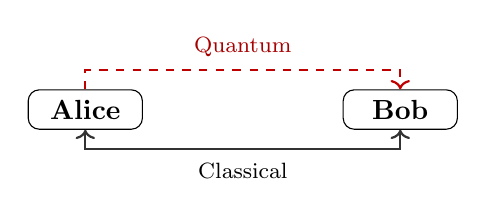
\begin{tikzpicture}
            \tikzset{
                party/.style={
                    draw,
                    rounded corners,
                    minimum width=1.45cm,
                    minimum height=0.5cm,
                    align=center,
                    font=\bfseries
                }
            }
            \tikzset{
                qcomm/.style={
                    red!75!black,
                    dashed,
                    thick
                }
            }
            \tikzset{
                ccomm/.style={
                    black!60!gray,
                    thick
                }
            }

            \node[party] (A) at (-2,0) {Alice};
            \node[party] (B) at (2,0) {Bob};
            
            \node[] (J) at (0, 0.5) {};
            \node[above=5pt of J.south, font=\footnotesize, align=center, red!65!black] {Quantum};
            
            \node[] (K) at (0, -0.5) {};
            \node[below=5pt of K.north, font=\footnotesize, align=center] {Classical};

            \draw[-,qcomm] (A.north) |- (J);
            \draw[->,qcomm] (J.west) -| (B.north);

            \draw[->,ccomm] (K.west) -| (A.south);
            \draw[->,ccomm] (K.west) -| (B.south);
        \end{tikzpicture}
        \caption{Communication diagram for point-to-point BB84}
        \label{bb84_comm}
    \end{subfigure}

    \vspace{6mm}
    \begin{subfigure}
        \centering
        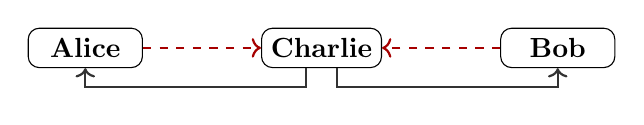
\begin{tikzpicture}
            \tikzset{
                party/.style={
                    draw,
                    rounded corners,
                    minimum width=1.45cm,
                    minimum height=0.5cm,
                    align=center,
                    font=\bfseries
                }
            }
            \tikzset{
                qcomm/.style={
                    red!65!black,
                    dashed,
                    thick
                }
            }
            \tikzset{
                ccomm/.style={
                    black!60!gray,
                    thick
                }
            }

            \node[party] (A) at (-3,0) {Alice};
            \node[party] (B) at (3,0) {Bob};
            \node[party] (C) at (0,0) {Charlie};

            \draw[->,qcomm] (A.east) -- (C.west);
            \draw[->,qcomm] (B.west) -- (C.east);

            \node[] (J) at (-1.5,-0.5) {};
            \node[] (K) at (1.5, -0.5) {};

            \draw[-,ccomm] ($(C.south)+(-0.2,0)$) |- (J.west);
            \draw[-,ccomm] ($(C.south)+(0.2,0)$) |- (K.east);
            \draw[->,ccomm] (J) -| (A.south);
            \draw[->,ccomm] (K) -| (B.south);
        \end{tikzpicture}
        \caption{Communication diagram for point-to-point MDI. Alice-Charlie and Bob-Charlie communication mirrors BB84.}
        \label{mdi_comm}
    \end{subfigure}
\end{figure}

MDI's shift of paradigm to use entanglement in its measurements removes the need for security assumptions around the trustworthiness of detectors. If Eve had control of Charlie's relay station in MDI, she could ascertain information about the interaction between the polarisations of photons (or other encoding), but not the pure polarisations itself. This differs from BB84, where polarisation is measured directly. The case for and provability of MDI's security (beyond the original security proof in \cite{Lo_2012}) is laid out in \cite{Primaatmaja2019} through a versatile security framework. Equivalent to EB methods, which do not protect against detector-side threats, in time-reversal once again, MDI remains open to source-side vulnerabilities. As is universal across deployments of QKD, nor is it impervious to implementation imperfections. Hardware-aware MDI vulnerabilities such as those in \cite{GU20222167} present a real-terms threat, where flawed and correlated sources can lead to weakened key security, and \cite{Lu:23} demonstrates a counterpoint to MDI security claims. MDI is not, in general, unconditionally secure (as with any physical realisation of a QKD system) and remains susceptible to implementation attacks both in theory and practice.

\begin{figure}[h]
    \begin{subfigure}
        \centering
        \includegraphics[width=0.8\linewidth]{img/bb84-mdi-kr.png}
        \caption{The comparison of the ultimate key rate between the finite standard BB84 protocol [13] (solid line) and finite MDI QKD (dashed line) when both have a number of sifted data equal to $10^{10}$. When the number of clicks received by Bob is $10^{10}$ in the finite BB84 protocol, the ultimate key rate is given by dash-dotted line. Courtesy of \cite{Song-2012}.}
        \label{fig:mdi_kr_bb84}
    \end{subfigure}
    \begin{subfigure}
        \centering
        \includegraphics[width=0.8\linewidth]{img/mdi_kr.png}
        \caption{Comparative lower bounds on key rate for MDI-QKD (green) and EB protocol (red), courtesy of \cite{Lo_2012}. Realistic and unified parameters such as loss, detection efficiency, dark counts and more are assumed. Noting EB schemes present a rate reduction relative to BB84, MDI does too by extension.}
        \label{fig:mdi_kr_eb}
    \end{subfigure}
\end{figure}

\subsection*{Scope and Theoretical Bounds}
Choosing which protocol to implement, however, demands more than security analysis: any deployment decision must account for how close a given hardware configuration can come to a theoretical ceiling on key rate, and whether the chosen protocol's rate-distance scaling makes it viable at the target distance.

The distance a quantum channel can span with sufficient quantum state survival rate is physically limited by photon attenuation across fibre lengths (or factors like atmospheric turbulence in free space). To counter this, quantum repeaters provide methods to extend maximal communication distances by storing and swapping entanglement to chain identical quantum states.

Core to the rich research landscape of QKD, Pirandola et al. provide a fundamental result in \cite{Pirandola_2017}, presenting a universal bound on maximally achievable secure key rates for repeater-less quantum communications, known as the PLOB bound. The bound establishes that at best, a point-to-point (P2P), no repeater, QKD scheme's key rate scales negative-linearly with channel transmittance (and thus negative-exponentially in distance), or the ratio of optical flux input that is transmitted through the channel, as $\mathcal{O}(\eta)$. Both BB84 and standard MDI are subject to this bound, but twin-field (TF) QKD \cite{Lucamarini_2018}, as proposed in 2018 by Lucamarini et al. using MDI's core tenet of an untrusted central relay node, is able to outperform PLOB by replacing the two-photon BSM with single-photon interference. As a result, key rates scale as $\mathcal{O}(\sqrt{\eta})$, an improvement as transmittances lie in the interval $(0,1)$.

The question of whether MDI-QKD could itself ever exceed the PLOB bound is more subtle. PLOB's derivation assumes a direct, two-way assisted (by a relay) point-to-point channel with no entanglement across photon shots from the same source. Crucially, it assumes that the relay performs a measurement which contributes no net entanglement generation between Alice and Bob. While MDI employs BSMs, these do not contribute net entanglement between Alice and Bob. Assuming end users can be trusted, they do not retain copies of 
\begin{figure}[h]
    \centering
    \includegraphics[width=0.8\linewidth]{img/PLOB_bound.png}
    \caption{The PLOB bound against various QKD schemes in idealised parameter conditions (with 0.2 dB/km loss), image courtesy of \cite{Pirandola_2017}. MDI sacrifices key rate for its security advantage.}
    \label{fig:PLOB}
\end{figure}
\noindent the photons they send to Charlie. Even assuming they cannot be trusted, Charlie's subsequent measurement, which is all complete before the raw key is output, collapses any potential entanglement. Assuming Charlie performs as we have directed him to, PLOB bounds MDI's peak performance, Fig. \ref{fig:PLOB}.

The path to exceeding PLOB key rates in an MDI setting therefore requires relaxing the two-photon coincidence requirement, precisely what TF-QKD achieves through single-photon interference. Alternatively, through more recent proposals such as post-measurement pairing QKD (PMP-QKD, \cite{Xie2022} and \cite{zeng2022} independently), which retains MDI's structure but allows Alice and Bob to pair their photons (where pairing is in the MDI sense post-BSM announcement) after detection within a coincidence window, users can increase the number of usable detection events beyond what the PLOB bound permits.

Continuous-Variable (CV) QKD, originally formulated in the early 2000's by Grosshans and Grangier \cite{GG02}, presents a class of protocols that instead employ continuous variables like phase and amplitude of an electromagnetic field to perform their bit encodings. Measurement-Device-Independence has been extended to the CV realm, producing a class of protocols that retain the security advantage of an untrusted relay whilst encoding information continuously. CV-MDI-QKD, proposed in 2015 by Pirandola et al. \cite{Pirandola_2015}, and reviewed in detail in \cite{Pirandola_2020}, operates by having Alice and Bob each prepare coherent states drawn from a Gaussian modulation and transmit these to Charlie. He subsequently performs a joint continuous-variable Bell measurement by mixing the two incoming modes on a beam-splitter, and communicates the outcomes classically to the end nodes. While CV-MDI-QKD and twin-field variants represent important extensions of the MDI paradigm to raise key rates or loosen hardware requirements (CV allows for off-the-shelf components), the remainder of this review focuses on DV-MDI-QKD implementations using discrete polarisation-encoded qubits, with this the dominant experimental and commercial implementation to date. BB84 is retained as a reference point for performance and realisation comparison.

\section{Hardware and Physical Layer}
\label{sect:hardware}
BB84 and MDI use identical qubit architectures, or physical implementations of quantum states. As is common across all of QKD, photons are currently the only viable quantum states for transmission, as they travel at the speed of light, interact weakly with their environment and slot naturally into existing classical optical communications infrastructure. The ways that bits and keys are represented in quantum information-theoretic objects is their encoding. The original papers for both BB84 and MDI utilised polarisation-encoded qubits, though others have expanded both protocols to employ a variety of encoding methods. These include phase (relative phase between components of the wavefunction, see \cite{Townsend1993}, \cite{Tamaki_2012}) and time-bin (time slot of photon arrival, see \cite{Brendel_1999}, \cite{Woodward_2021}) encoding, or a combination of the two (\cite{Liu2013}). More niche methods beyond include frequency-bin (\cite{Tagliavacche_2025}) and orbital angular momentum (\cite{Zhou_2016}, \cite{Vallone_2014}).

In Lo et al.'s exposition of MDI-QKD, Weak Coherent Pulse (WCP) lasers are used as qubit sources, where the number of photons emitted in one window is random (following a Poisson distribution). At the time of the paper's writing, WCPs were the most reliable and cost effective way to generate quantum communications-ready polarised photons, and deterministic single-photon sources (discussed in sections to follow) were not commercially available. These sources raise their own vulnerabilities - most pressing of which being the Photon Number Splitting (PNS) attack \cite{PNS_desc}, \cite{Avanesov2025}. Multi-photon pulses emitted by these sources are susceptible to having trailing photons removed from the transmission by Eve. She holds onto these until the bases are announced by Alice and Bob, and can successfully measure the photon without disturbing the state. Through this she is able to hold some portion of Alice and Bob's shared key against their knowledge and without exceeding the QBER. To mitigate these attacks, additional complexity is incorporated to sources through decoy-state encoding, in both MDI-QKD and BB84, also demonstrated for the first time by Lo \cite{Lo_decoys} in 2005. In decoy-state QKD, photon transmitters vary the mean photon number between a signal intensity and one or more lower ``decoy" intensities, keeping the choice secret from Eve. By comparing measurement statistics across intensities, end users can tightly bound single-photon pulse contributions to their key and estimate Eve's information accurately, optimising key rates in spite of imperfect sources.

In spite of this additional vulnerability, optimal secure distance and key rates have been pushed with such sources. Yin et al.'s result in 2016 \cite{Yin_2016} demonstrated a decoy-state MDI scheme achieving secure distance of 404km, using ultra-low-loss fibre, representing decoy-state MDI's current practical ceiling. The pursuit of greater distances and rates \textit{not} at the cost of reduced security has pushed the research of alternative photon sources. The decoy-state paradigm presents the exact same vulnerabilities to BB84, though with two independent sources per key-generation event rather than one, MDI doubles the attack surface for PNS relative to BB84.

\subsection*{Single Photon Sources}
Since MDI's inception in 2012, Single Photon Sources (SPSs) have received a huge amount of research \cite{SPS_history} and commercialisation \cite{first_SPS}, \cite{QuandelaSPS}. Brassard et al.'s 2000 paper \cite{Brassard_2000} brought SPSs to the forefront of QKD through their exposition of the enhanced security obtained 
\begin{figure}[h]
    \begin{subfigure}
        \centering
        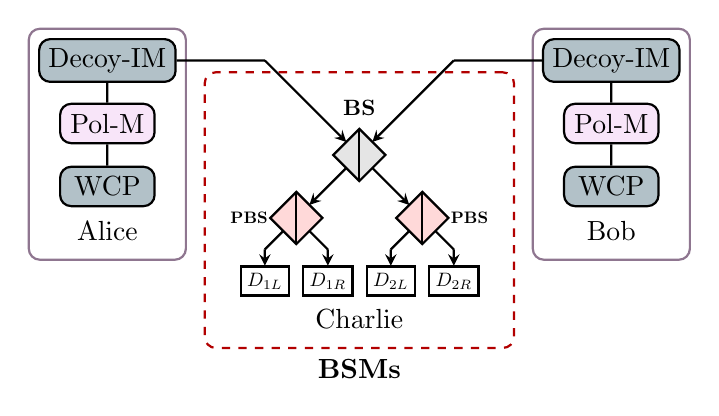
\begin{tikzpicture}[>=stealth,thick,scale=0.8,align=center]
            \tikzset{
                hardware/.style={
                    draw,
                    rounded corners,
                    minimum width=1.2cm,
                    minimum height=0.5cm,
                    align=center
                }
            }
    
            % Alice Optics
            \node[hardware,fill=lightgray] (A_WCP) at (-4,-0.5) {WCP};
            \node[hardware,fill=purple!15] (A_PolM) at (-4,0.5) {Pol-M};
            \node[hardware,fill=lightgray] (A_Decoy) at (-4,1.5) {Decoy-IM};
            \node[] (A) at (-4,-1.2) {Alice};
    
            \draw[-, thick] (A_WCP) -- (A_PolM);
            \draw[-, thick] (A_PolM) -- (A_Decoy);
    
            \node[
                draw,
                purple!20!gray,
                rounded corners,
                fit = (A_WCP) (A_PolM) (A_Decoy) (A),
            ] (A_Box) {};
    
            % Bob Optics
            \node[hardware,fill=lightgray] (B_WCP) at (4,-0.5) {WCP};
            \node[hardware,fill=purple!15] (B_PolM) at (4,0.5) {Pol-M};
            \node[hardware,fill=lightgray] (B_Decoy) at (4,1.5) {Decoy-IM};
            \node[] (B) at (4,-1.2) {Bob};
    
            \draw[-, thick] (B_WCP) -- (B_PolM);
            \draw[-, thick] (B_PolM) -- (B_Decoy);
    
            \node[
                draw,
                purple!20!gray,
                rounded corners,
                fit = (B_WCP) (B_PolM) (B_Decoy) (B),
            ] (B_Box) {};
    
            % Charlie Optics
            %% Beam Splitter
            \node (BS_T) at (0,0.25) {};
            \node (BS_B) at (0,-0.25) {};
            \node (BS_R) at (0.25,0) {};
            \node (BS_L) at (-0.25,0) {};
    
            \draw[thick,fill=gray!20]
                (BS_T.north) -- node[midway] (incoming_B) {}
                (BS_R.east)  -- node[midway] (outgoing_R) {}
                (BS_B.south) -- node[midway] (outgoing_L) {}
                (BS_L.west)  -- node[midway] (incoming_A) {} cycle;
            \draw[-] (BS_B.south) -- (BS_T.north);
    
            \node[scale=0.8] (BS_label) at (0,0.75) {\textbf{BS}};
    
            \node[
                fit=(BS_T) (BS_B) (BS_R) (BS_L) (BS_label),
            ] (BS) {};
    
            %% Polarising Beam Splitters
            %%% Left
            \node (PBS1_T) at (-1,-0.75) {};
            \node (PBS1_B) at (-1,-1.25) {};
            \node (PBS1_R) at (-0.75,-1) {};
            \node (PBS1_L) at (-1.25,-1) {};
    
            \draw[thick,fill=red!15]
                (PBS1_T.north) -- node[midway] (in_PBS1) {}
                (PBS1_R.east)  -- node[midway] (out_1R) {}
                (PBS1_B.south) -- node[midway] (out_1L) {}
                (PBS1_L.west)  -- cycle;
            \draw[-] (PBS1_T.north) -- (PBS1_B.south);
    
            \node[scale=0.6] (PBS1_label) at (-1.75,-1) {\textbf{PBS}};
    
            \node[
                fit=(PBS1_T) (PBS1_B) (PBS1_R) (PBS1_L) (PBS1_label),
            ] (PBS1) {};
    
            %%% Right
            \node (PBS2_T) at (1,-0.75) {};
            \node (PBS2_B) at (1,-1.25) {};
            \node (PBS2_R) at (1.25,-1) {};
            \node (PBS2_L) at (0.75,-1) {};
    
            \draw[thick,fill=red!15]
                (PBS2_T.north) --
                (PBS2_R.east)  -- node[midway] (out_2R) {}
                (PBS2_B.south) -- node[midway] (out_2L) {}
                (PBS2_L.west)  -- node[midway] (in_PBS2) {} cycle;
            \draw[-] (PBS2_T.north) -- (PBS2_B.south);
    
            \node[scale=0.6] (PBS2_label) at (1.75,-1) {\textbf{PBS}};
    
            \node[
                fit=(PBS2_T) (PBS2_B) (PBS2_R) (PBS2_L) (PBS2_label),
            ] (PBS2) {};
    
            %%% Connecting to BS
            \draw[->,thick] (outgoing_L.center) -- (in_PBS1.center);
            \draw[->,thick] (outgoing_R.center) -- (in_PBS2.center);
    
            %% Detectors
            \node[draw,scale=0.7] (D1L) at (-1.5,-2) {$D_{1L}$};
            \node[draw,scale=0.7] (D1R) at (-0.5,-2) {$D_{1R}$};
    
            \node[draw,scale=0.7] (D2R) at (1.5,-2) {$D_{2R}$};
            \node[draw,scale=0.7] (D2L) at (0.5,-2) {$D_{2L}$};
    
            %% PBS-Detector Connections
            \draw[-,thick] (out_1L.center) -- (-1.5,-1.5);
            \draw[->,thick] (-1.5,-1.5) -- (D1L.north);
            \draw[-,thick] (out_1R.center) -- (-0.5,-1.5);
            \draw[->,thick] (-0.5,-1.5) -- (D1R.north);
    
            \draw[-,thick] (out_2L.center) -- (0.5,-1.5);
            \draw[->,thick] (0.5,-1.5) -- (D2L.north);
            \draw[-,thick] (out_2R.center) -- (1.5,-1.5);
            \draw[->,thick] (1.5,-1.5) -- (D2R.north);
    
            \node[
                fit=(D1L) (D1R) (D2L) (D2R),
            ] (Detectors) {};
    
            \node (C) at (0,-2.6) {Charlie};
    
            \node[
                draw,
                thick,
                dashed,
                red!70!black,
                rounded corners,
                fit = (BS) (PBS1) (PBS2) (Detectors) (C),
                label = {below:\textbf{BSMs}}
            ] (A_Box) {};
    
            % Alice/Bob-Charlie communication
            \draw[-,thick] (A_Decoy.east) -- (-1.5,1.5);
            \draw[->,thick] (-1.5,1.5) -- (incoming_A.center);
            \draw[-,thick] (B_Decoy.west) -- (1.5,1.5);
            \draw[->,thick] (1.5,1.5) -- (incoming_B.center);
        \end{tikzpicture}
        \caption{Optical implementation of MDI-QKD, adapted from Lo et al. \cite{Lo_2012}. Alice and Bob prepare BB84 states, which interfere at a $50\colon50$ beam splitter inside Charlie's relay. Outputs of this are projected onto horizontal and vertical polarisations and detected.}
        \label{fig:optical_mdi}
    \end{subfigure}
    \vspace{0.3cm}
    \begin{subfigure}
        \centering
        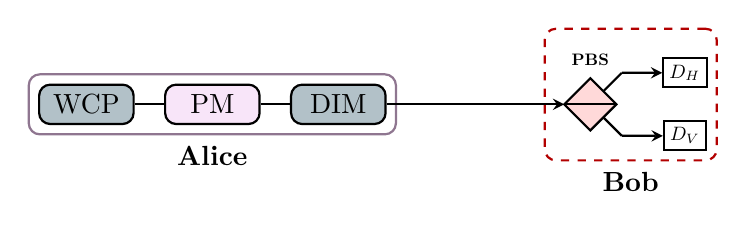
\begin{tikzpicture}[>=stealth,thick,scale=0.8,align=center]
            \tikzset{
                hardware/.style={
                    draw,
                    rounded corners,
                    minimum width=1.2cm,
                    minimum height=0.5cm,
                    align=center
                }
            }
    
            % Alice Optics
            \node[hardware,fill=lightgray] (A_WCP) at (-4,0) {WCP};
            \node[hardware,fill=purple!15] (A_PolM) at (-2,0) {PM};
            \node[hardware,fill=lightgray] (A_Decoy) at (0,0) {DIM};
    
            \draw[-, thick] (A_WCP) -- (A_PolM);
            \draw[-, thick] (A_PolM) -- (A_Decoy);
    
            \node[
                draw,
                purple!20!gray,
                rounded corners,
                fit = (A_WCP) (A_PolM) (A_Decoy),
                label = {below:\textbf{Alice}}
            ] (A_Box) {};
    
            % Bob Optics
            \node (PBS1_T) at (4,0.25) {};
            \node (PBS1_B) at (4,-0.25) {};
            \node (PBS1_R) at (4.25,0) {};
            \node (PBS1_L) at (3.75,0) {};
    
            \draw[thick,fill=red!15]
                (PBS1_T.north) -- node[midway] (out_T) {}
                (PBS1_R.east)  -- node[midway] (out_B) {}
                (PBS1_B.south) -- node[midway] (waste) {}
                (PBS1_L.west)  -- cycle;
            \draw[-] (PBS1_L.west) -- (PBS1_R.east);
    
            \node[scale=0.6] (PBS1_label) at (4,0.7) {\textbf{PBS}};
    
            \node[
                fit=(PBS1_T) (PBS1_B) (PBS1_R) (PBS1_L) (PBS1_label),
            ] (PBS1) {};
    
            %% Detectors
            \node[draw,scale=0.7] (DH) at (5.5,0.5) {$D_{H}$};
            \node[draw,scale=0.7] (DV) at (5.5,-0.5) {$D_{V}$};

            \node[
                draw,
                thick,
                dashed,
                red!70!black,
                rounded corners,
                fit = (PBS1) (DH) (DV),
                label = {below:\textbf{Bob}}
            ] (Bob) {};

            \draw[->, thick] (A_Decoy) -- (PBS1_L);
            \draw[-, thick] (out_T.center) -- (4.5,0.5);
            \draw[-, thick] (out_B.center) -- (4.5,-0.5);
            \draw[->, thick] (4.5,0.5) -- (DH);
            \draw[->, thick] (4.5,-0.5) -- (DV);
        \end{tikzpicture}
        \caption{Optical implementation of decoy-state BB84, modelled after the diagram of Lo et al. Alice's node contains the same component sequence as in MDI.}
        \label{fig:optical_bb84}
    \end{subfigure}
\end{figure}
\noindent in BB84 when using Parametric Down Conversion (PDC) to generate individual photons. By exploiting a nonlinear optical process in which one high-energy pump photon is split into a pair of lower-energy entangled photons, detection of one heralds the presence of its twin with high fidelity, registering a single photon. PDC is a practically attractive route to QKD-focused single-photon emission, since it allows the transmitting party to post-select on successful generation events and thereby substantially reduce WCP multi-photon emission probability. The security argument is correspondingly strengthened, as Eve cannot intercept trailing photons from pulses she knows to be multi-photon without Alice registering a heralding event.

PDC sources are inherently probabilistic: photon pairs are generated according to a Poissonian process, and operating at mean pair-number well below one per pulse, to limit PNS attacks, necessarily constrains the achievable key rate. This intrinsic security-rate trade-off motivated subsequent research into deterministic single-photon emitters, of which quantum dots represent the most mature platform \cite{Bozzio_2022}, \cite{Yang_2024}.

Papers since have sought to integrate SPSs into the literature surrounding MDI-QKD, demonstrating both applicability to the setting and their role in improving maximum secure distance and secure key rate. Zhou et al.'s results \cite{Zhou_2018} in 2018 demonstrated via numerical simulation a 100x improvement to the secure key rate using quantum blockades as the source, and Zhan et al. demonstrated \cite{Zhan2023} in 2023 an optimisation model (validated through simulation) for Spontaneous PDC sources (SPDCs) that greatly improves the key rate with such sources. The same authors (plus one) experimentally achieved in 2025 improved synchronisation of photon arrival (discussed further below) at the relay node \cite{Zhan2025} with Heralded SPSs (HSPSs), subsequently increasing key rate and transmission distance. Bozzio et al. establish theoretically the validity of Quantum Dots (QDs) in QKD schemes \cite{Bozzio_2022} given their ability to emit deterministically, in principle, with high brightness and low multi-photon emission rate. The authors show that even when WCP sources are given the most favourable decoy-state treatment (infinite decoy intensities), QD sources with modest generation success rates are able to outperform over long distances. One of MDI's benefits over BB84 is the extension of secure distance, and QDs would compound this.

\subsection*{Measurement of Interaction}
\label{sect:interaction}
Unlike in BB84, MDI's detectors measure for metrics of polarisation interaction, or entanglement, rather than individual photon polarisation. Fig. \ref{fig:bsm_circ} gives a circuit representation in quantum information-theoretic terms of such a measurement. To achieve this entanglement measurement optically in \cite{Lo_2012}, the authors employ a beam-splitter (BS) to perform the entangling operation, and polarising beam-splitters (PBS) to perform projections onto detectors. In Fig. \ref{fig:optical_mdi}, $D_{n,S}$ denotes the $n$th detector on the $S$-hand arm, Pol-M is the polarisation modulator applying the photon state encoding and Decoy-IM represents the decoy-state intensity modulator, varying the laser strength randomly.

This physical setup produces a detection event at one or more of the four detectors for each incoming photon pair. The BSM outcome is not the raw detector click(s) as in BB84, but the result of a coincidence logic applied across the array. Generally, a valid Bell state detection requires precisely two simultaneous (within a coincidence window) detector clicks such that the joint event can be attributed to a distinguishable Bell state rather than noise or multi-photon contamination. In the linear-optic BSM of Lo et al. \cite{Lo_2012}, constructed from a single BS and two PBSs, it is well established that only two of the four Bell states, $|\psi^{+}\rangle$ and $|\psi^{-}\rangle$, are unambiguously distinguishable, corresponding to specific cross-arm coincidence patterns at the 
\begin{figure}[h]
    \centering
    \begin{quantikz}
            \lstick{$q_0$} & \ctrl{1} & \gate{H} & \meter{} \\
            \lstick{$q_1$} & \targ{}  &          & \meter{}
    \end{quantikz}
    \caption{BSM circuit in abstract quantum information terms - entangling \texttt{CNOT} gate (bit-flip $q_1$ if $q_0$ in $\ket{1}$ state) followed by \texttt{Hadamard} gate (map computational basis to X-basis and vice versa) and subsequent measurements.}
    \label{fig:bsm_circ}
\end{figure}
detector pairs. Concretely, a $|\psi^{+}\rangle$ projection is registered when $D_{1L}$ and $D_{1R}$ fire, or when $D_{2L}$ and $D_{2R}$ fire, whilst $|\psi^{-}\rangle$ corresponds to the cross-polarisation coincidences $D_{1L}$ and $D_{2R}$, or $D_{1R}$ and $D_{2L}$. This incomplete distinguishability is a result of the Hong-Ou-Mandel (HOM) effect \cite{Hong_1987}: the idea that two indistinguishable photons arriving simultaneously at a beam-splitter will always leave together (see Fig. \ref{fig:hom_eff} for validation). Single-
\begin{figure}[h]
    \centering
    \includegraphics[width=0.8\linewidth]{img/hong_ou_mandel.png}
    \caption{Experimental demonstration of the Hong-Ou-Mandel effect, courtesy of \cite{Lo_2012}. Coincidence count reaches a minimum when photons arrive simultaneously.}
    \label{fig:hom_eff}
\end{figure}
\noindent detector events and same-arm (both $L$ or both $R$) coincidences are discarded as inconclusive. The maximum fraction of useful detection events in this setup is therefore capped at 50\% - a fundamental constraint of the optical implementation that directly limits the sifted key rate, independently of channel loss. This realisation of the HOM effect has motivated proposals for enhanced BSM designs using auxiliary photons or non-linear optical elements such as \cite{Pirandola_2020}.

BB84, on the other hand, has zero coincidence logic in the post-measurement and consists of a direct single-photon polarisation reading at Bob's node. Further, as only one photon is measured, there are no indistinguishability concerns as in the HOM effect, removing the 50\% efficiency cap that MDI experiences. This is the central hardware asymmetry between the two protocols.

\subsection*{Source Synchronisation}
MDI-QKD introduces a requirement for source synchronisation. In order to perform a BSM with high fidelity at the relay, practical realisations of the protocol must ensure that photons arrive at the same time, or within a suitably small coincidence window, to allow entanglement. In practice, in an MDI scheme, Alice and Bob are spatially separated, their sources are physically independent, and optical path lengths to Charlie will differ. A temporal mismatch degrades the visibility of the HOM effect at the relay's beam-splitter. A reduction in HOM visibility translates directly into a reduction in the fraction of detection events attributable to a definite Bell state, thereby increasing the effective QBER and reducing key rate. Synchronisation in MDI-QKD is achieved through a combination of classical clock distribution and active optical feedback. Tuning path lengths and source wavelengths against the HOM coincidence rate maintains the photon indistinguishability required for high-fidelity BSMs, as Tang et al. address in a deployed setting \cite{Tang_2016}. Zhan et al. \cite{Zhan2025} address this directly through the use of HSPSs, in which the detection of an idler photon from a PDC source serves as a herald that triggers the relay to open its coincidence window precisely when a signal photon is in transit from each end node. By conditioning measurement events on heralding signals from both Alice and Bob, the authors demonstrate experimentally that photon arrival synchronisation can be substantially improved, yielding increases in both secure key rate and transmission distance. This additional level of complexity, however, is one not required in PM schemes, as single-photon detection requires a single measurement and no additional timing requirements are imposed.

\subsection*{Chip-Based QKD}
A number of authors have sought to miniaturise QKD systems. Sibson et al. present the first miniaturised and reconfigurable integrated device implementing QKD \cite{sibson2015}: their InP platform demonstrated a proof of concept for miniaturisable QKD. In \cite{Semenenko:20}, secure MDI key exchange up to 200 km is presented, using mass-manufacturable integrated InP-chip-based transmitters. Both works reduce the barrier for widespread QKD adoption by presenting accessible and secure platforms. Alternative substrates are also offered by Wei et al. \cite{Wei_2020}, who demonstrate experimentally high secure MDI key rates over 180km of standard fibre using Si chips. Hardware is evolving from the original bulk optics used in 2012 to miniaturisable, cost-efficient integrated photonics, pushing forward the commercial landscape and appetite for QKD systems and their integration into existing infrastructure. Fig.'s \ref{fig:chip-based-bb84} and \ref{fig:chip-based-mdi} show relevant chip-based setups for BB84 and MDI-QKD, respectively.

\begin{figure}[h]
    \begin{subfigure}
        \centering
        \includegraphics[width=0.9\linewidth]{img/chip-based-bb84.png}
        \caption{Chip-based BB84 photon transmitter and receiver, as presented in \cite{sibson2015}. (a) and (b) are the transmitter and receiver, respectively, while other inlays show masks and circuitry of the chips.}
        \label{fig:chip-based-bb84}
    \end{subfigure}
    \begin{subfigure}
        \centering
        \includegraphics[width=0.9\linewidth]{img/chip-based-mdi.png}
        \caption{Chip-based MDI-QKD photon transmitters and relay station, as presented in \cite{Cao2020_chipbased}. Components in both transmitters and relay map easily to the optical components in Lo et al.'s original exposition. A phase modulator allows for phase-encoding. The signal passes through a path-to-polarisation converter (PPC) and is transmitted to Charlie's electrically driven polarisation converter (EPC).}
        \label{fig:chip-based-mdi}
    \end{subfigure}
\end{figure}

\subsection*{Transmission Channels}
Beyond sources, MDI is not conducive to free space transmission in the same way that PM schemes are due to the need for photon arrival synchronisation in both space and time. Atmospheric turbulence and high background noise offer considerable challenge to this requirement, as discussed by Cao et al. in \cite{Cao2020}. As such, MDI is largely limited to fibre links for transmission, though significant research has been done to understand how we may integrate MDI into existing classical communications networks.

Townsend, Rarity and Tapster's 1993 experiment \cite{Townsend1993} demonstrated the first prototype for a single-photon combined polariser and transmission channel with: operating wavelength in the O-band ($1.3\mu\text{m}$), 10 km fibre transmission and fringe visibility greater than 90\%. The work laid out proof of concept of QKD's potential to exist and operate through currently in-service commercial fibre. Work like Patel et al.'s \cite{Patel_2012} extended this foundation to demonstrate high QKD bit-rates (up to 507 kbps) over 50km of fibre shared with error-free bidirectional data communications of rate in the Gbps range. The authors produced non-trivial key rate in such fibres up to 90km, up to 7.6 kbps, roughly a 6x speedup at the time. In 2022, Berrevoets et al. were able to generate, experimentally, a point-to-point MDI-QKD system existing on the same fibre links as 10 Gbps traditional IP connectivity \cite{Berrevoets_2022}. The team were able to field deploy and autonomously run an MDI link in the Netherlands for two weeks, with end nodes separated from the relay by 14.7 and 10.2 km of fibre. They also showed, by simulation, that 200 Gbps classical links would only decrease secure quantum key rate by a factor of 2 - though significant experimental improvement would be required for such throughput.

This all being said, QKD links sharing physical space with telecom signals presents a number of open challenges. Principal of these is Raman scattering \cite{Raman_1928}, a phenomenon by which photons are inelastically scattered by matter, and the effect's extent on a signal is an intrinsic material property. Photons' frequencies are shifted by up to 200 nm in silicon fibre, at a rate of around one in every million, though in classical communications of data rate 10 Gbps, this corresponds to 10,000 photons scattered due to the effect per second. For QKD links living in the same channel as such low data rates, any scattered photons from the classical communication arriving at a detector in the same time-bin as expected QKD photons can cause fake detections, artificially inflating the QBER. The wavelength range in silicon is broad enough to contaminate quantum channels regardless of fibre spectrum partition. Chapuran et al., in \cite{Chapuran_2009}, identified for the first time the class of Raman 
\begin{figure}[h]
    \centering
    \includegraphics[width=\linewidth]{img/ramanscattering-fig1.png}
    \caption{Light incident on matter can undergo three varieties of scattering: that producing light of equal, shorter or longer wavelength - Raman scattering changes the wavelength of scattered light. Diagram courtesy of \cite{Raman_scatter}.}
    \label{fig:raman}
\end{figure}
\noindent scattering that presents the dominant interference with general QKD's existence with classical channels (Anti-Stokes Raman Scattering in Fig. \ref{fig:raman}), and the problem is characterised experimentally in great detail in \cite{daSilva_2014}. Since, a temporal filtering technique characterised in \cite{Patel_2012} presents the primary mitigation technique for QKD systems coexisting with classical fibre. More recently, Wu et al. \cite{Wu2025} give a state-of-the-art demonstration of field-deployed QKD coexistence with 110.8 Tbps classical traffic by using multi-core fibres (MCFs). The authors model the inter-core scattering to give the first deployed MCF with industry standard cladding co-operating DV-QKD with high-throughput C-band telecoms data.

These challenges are not unique to MDI-QKD, and BB84, in using the same fibre infrastructure, would likewise be subject to Raman scattering. MDI, however, and somewhat counter-intuitively, is more resilient to such effects. In Valivarthi et al.'s paper \cite{valivarthi-2019}, demonstrate that, due to needing to detect two photons per key bit, the effect of Raman noise on MDI-QKD is lessened in relation to BB84. The effects of noise along two shorter paths appear to ``compose" to create a total noise effect less than that along the concatenation of the path, providing a performance boost to MDI.

\section{Network Architectures}

Wavelength Division Multiplexing (WDM) presents a natural mechanism for scaling QKD systems from point-to-point links to multi-user networks without a proportional increase in physical fibre infrastructure required. In the WDM architecture, multiple quantum channels associated with distinct wavelengths are co-propagated along a single fibre, allowing a shared physical medium to serve multiple pairs 
\begin{figure}
    \centering
    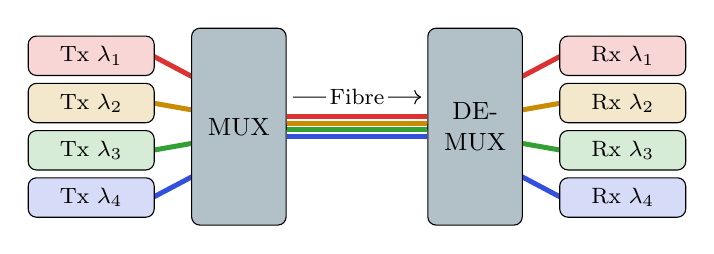
\begin{tikzpicture}[scale=0.75]
        % -- Multiplexer -----------------------------------------------
        \node[draw, fill=lightgray,rounded corners=3pt,
            minimum width=1.2cm, minimum height=2.5cm,
            align=center, font=\small]
            (mux) at (-2,0) {MUX};
        % -- Transmitter channels (left) -------------------------------
        \foreach \i/\clr/\lam in {1/wl1/\lambda_1, 2/wl2/\lambda_2,
                                  3/wl3/\lambda_3, 4/wl4/\lambda_4}{
            \node[draw, fill=\clr!20, rounded corners=3pt,
              minimum width=1.6cm, minimum height=0.5cm,
              align=center, font=\footnotesize]
            (tx\i) at (-4.5, -\i*0.8 + 2)
            {Tx $\lam$};
            \begin{pgfonlayer}{background}
                \draw[-,\clr,line width=1.8pt] ([xshift=-1pt]tx\i.east) -- (mux.east);
            \end{pgfonlayer}
        }

        % -- De-multiplexer --------------------------------------------
        \node[draw, fill=lightgray,rounded corners=3pt,
            minimum width=1.2cm, minimum height=2.5cm,
            align=center, font=\small]
            (demux) at (2,0) {DE-\\MUX};
        % -- Receiver channels (right) ---------------------------------
        \foreach \i/\clr/\lam in {1/wl1/\lambda_1, 2/wl2/\lambda_2,
                                  3/wl3/\lambda_3, 4/wl4/\lambda_4}{
            \node[draw, fill=\clr!20, rounded corners=3pt,
              minimum width=1.6cm, minimum height=0.5cm,
              align=center, font=\footnotesize]
            (rx\i) at (4.5, -\i*0.8 + 2)
            {Rx $\lam$};
            \begin{pgfonlayer}{background}
                \draw[-,\clr,line width=1.8pt] ([xshift=1pt]rx\i.west) -- (demux.west);
            \end{pgfonlayer}
            \draw[-,\clr,line width=1.8pt] ([yshift={(-2*\i+5)*1.6pt}]mux.east) -- ([yshift={(-2*\i+5)*1.6pt}]demux.west);
        }

        \node[font=\footnotesize] (fibre) at (0,0.5) {Fibre};
        \draw[-] ([xshift=3pt,yshift=0.5cm]mux.east) -- ([xshift=3pt]fibre.west);
        \draw[->] ([xshift=-3pt]fibre.east) -- ([xshift=-3pt,yshift=0.5cm]demux.west);
    \end{tikzpicture}
    \caption{Light of different wavelengths enters the Multiplexer (MUX), which passes this along a fibre. It is received by a De-Multiplexer (DE-MUX), which relays it on to the target nodes of each wavelength transmission.}
    \label{fig:WDM}
\end{figure}
\noindent of communicating parties simultaneously. The principle has a long lineage in quantum optical communications, and the noise environment for quantum-classical coexistence in such fibres has been examined for QKD in \cite{Peters_2009}. In MDI specifically, WDM is of particular architectural interest as the relay node must, by default, receive photons from multiple end users in a network setting; by assigning distinct wavelengths to various user pairs and demultiplexing at the relay, a single BSM apparatus can in principle serve an entire multiplexed network, reducing hardware overhead per user. WDM scaling for BB84 is a materially more simple engineering problem, as each wavelength covers an individual point-to-point link, whereas for MDI, synchronised photon arrival is required for every wavelength channel used in the fibre's spectrum.

Wengerowsky et al. \cite{Wengerowsky_2018} demonstrate experimentally a wavelength-multiplexed entanglement-based network, providing a conceptual template for WDM-MDI architectures at scale, noting again that MDI is EB's time-reversal. More recently, Xue et al. \cite{Xue2022} demonstrate MDI-QKD using frequency-nondegenerate (distinct frequencies) photon pairs, a proof-of-principle for WDM integration since the photons of the two communicating parties occupy distinct spectral slots by design. Yan et al. \cite{Yan2025} present a novel MDI network implementation built on an optical frequency comb, generating a coherent, phase-locked array of spectral modes, thus offering a scalable and highly stable WDM substrate for multi-user MDI-QKD. The technology slots in well to MDI, and its capacity to increase throughput renders it a natural candidate to guide MDI-QKD network design.

\subsection*{Trusted Nodes, Relays and Repeaters}
The dominant architecture in early QKD network deployments at scale was the trusted node model, in which point-to-point QKD links are chained with intermediate relay stations decrypting and re-encrypting key material in the classical domain before forwarding it toward its destination, for example in the DARPA \cite{Elliott_2002} and SECOQC \cite{Peev_2009} networks. The security of such networks is therefore only as strong as the physical and institutional security of each relay node - a significant operational liability in practice, particularly for deployments spanning jurisdictions or administered by multiple parties.

This motivated the search for relay architectures unreliant upon intermediate node trust, and in this context, MDI was a direct realisation of this aspiration. Arising with a qualitatively distinct security guarantee from the trusted node model, MDI-QKD is a compelling candidate for metropolitan and wide-area networks in which the relay may be co-located with or operated by an untrusted third party. Tang et al.'s field demonstration \cite{Tang_2016} over an untrustful metropolitan network is among the most direct experimental validations of this claim. Tang's architectural implication that relay hardware can be commercially procured and deployed without the burden of security certification carries significant weight for the practical economics of MDI infrastructure. As such, MDI provides significant advantage over BB84 from an operational perspective when scaling networks in distance, as it no longer necessitates a trusted-node model in the same way.

As regards performance, for a metropolitan QKD network, link length is not so far to necessitate use of trusted nodes and relays. As such, the greater key rate offered by BB84 without the required additional overheads (economic, operational and engineering, to name a few) renders it preferable over MDI in such localised settings, provided there are no requirements for the heightened security offerings that MDI brings.

Discussion of relay-based QKD naturally invites a note on quantum repeaters, whose eventual deployment would fundamentally alter the scaling landscape for long-distance QKD. Kimble's vision of the quantum internet \cite{Kimble_2008} frames repeaters as the essential enabling technology for a globally connected quantum communication network: by storing entanglement at intermediate nodes and performing entanglement swapping to extend it over arbitrary distances, a repeater chain could in principle overcome the exponential attenuation of photons in fibre. However, the practical realisation of quantum repeaters remains a substantially unsolved engineering problem, requiring long-lived quantum 
\begin{figure}[h]
    \centering
    \includegraphics[width=0.8\linewidth]{img/wehner_quantumInternet.jpeg}
    \caption{The three quantum hardware units essential to the quantum internet, as according to \cite{Wehner2018}: quantum channels to transmit, repeaters to extend range, and end nodes for usage.}
    \label{fig:wehner_internet}
\end{figure}
\noindent memories with high efficiency and low noise, together with fast and high-fidelity entanglement generation and classical feed-forward - none of which are currently available at the performance levels demanded by a useful repeater, as Kimble shows. In the near term, therefore, the relevant question for QKD deployment is how well repeater-free protocols perform against the PLOB bound \cite{Pirandola_2017}. Both BB84 and standard MDI-QKD are bounded by PLOB. Twin-field QKD \cite{Lucamarini_2018}, by exploiting single-photon interference at the relay rather than two-photon BSMs, achieves the reduced scaling that allows it to exceed PLOB and thus represents the most practically significant near-term stepping stone toward the performance levels at distance that would ultimately be delivered by a full quantum repeater.

\subsection*{Simulation of Metropolitan Networks}
Beyond point-to-point analysis, simulation has been employed to understand the behaviour of MDI-QKD at the metropolitan scale. Yehia et al. \cite{Yehia_2022} present the Quantum City framework, a simulation of a star-topology metropolitan quantum network in which a powerful central node serves a number of end users within limited hardware capabilities. The framework incorporates realistic physical parameters across components and simulates five distinct QKD configurations within the same architecture, among them MDI-QKD and entanglement-based QKD. The authors' results suggest that practical quantum-enhanced network functionalities are achievable with near-term hardware, though EB protocols (and similarly MDI) yield substantially lower key rates than PM schemes under current device parameters. The framework is of direct relevance to the comparative question motivating future work: by modelling multiple protocols within a common metropolitan topology and hardware condition, we aim to provide a template for controlled, multi-protocol simulation tailored to comparison of performance metrics.

\section{Deployed Systems and Testbeds}
\subsection*{BB84 Deployments}
The Tokyo QKD Network, reported by Sasaki et al. \cite{Sasaki_2011} and field-operational in 2010, represented at the time the most comprehensive multi-node, multi-vendor QKD testbed yet demonstrated. The network comprised six nodes connected by optical fibre links spanning distances of up to approximately 45 km, and incorporated QKD systems from four different manufacturers, visualised in Fig. \ref{fig:sasaki}. Each implements distinct physical encoding schemes, incorporating to form a unified key management architecture. The demonstration showed that one-time pad encrypted voice communications could be sustained continuously and securely across the network, including over links shared with conventional telecommunications traffic. From the perspective of network architecture, the Tokyo network remained a trusted-node deployment, with relay stations securing key material in the classical domain at each hop. Its principal contributions were therefore not in the security model but in operational maturity: the sustained, autonomous, multi-vendor operation of a heterogeneous QKD network over metropolitan-scale distances, over a period of months rather than days, constituted a 
\begin{figure}[h]
    \centering
    \includegraphics[width=0.95\linewidth]{img/sasaki2011_arch.jpeg}
    \caption{(a) Physical link configuration between various access points in the Tokyo QKD network, as in \cite{Sasaki_2011}. Six kinds of system are installed. (b) Logical link configuration with duplicated physical nodes where loop-backs are employed.}
    \label{fig:sasaki}
\end{figure}
\noindent qualitative step forward in demonstrating the commercial and infrastructural readiness of QKD technology. It also provided a detailed empirical dataset on the operational challenges of real-world QKD deployment, including timing synchronisation, wavelength management and key management protocol interoperability, that has informed subsequent network design efforts and remains a foundational reference for metropolitan QKD network architecture.

One of the largest QKD networks deployed to date is the Chinese integrated space-to-ground network reported by Chen et al. \cite{chen2021}, with terrestrial component spanning over 2,000 km of optical fibre and serving more than 150 industrial users across 4 major cities via trusted relay nodes. Integration with two satellite links, provided by the Micius quantum satellite, allows the network to achieve a combined reach of 4,600 km. Micius had already demonstrated the reach of satellite-based QKD independently: in 2018 it served as a trusted relay between ground stations in China and Austria, separated by approximately 7,600 km, in what was the first intercontinental quantum-secured videoconference, though a significant practical limitation was that the quantum states downloaded from the satellite required several days of post-processing to distil usable keys \cite{liao2018}. This limitation motivates the Jinan-1 programme, whose microsatellite payload weighs approximately 23 kg against Micius's substantially heavier infrastructure, operates a light source six times faster, and generates keys two to three orders of magnitude more quickly — enabling real-time key distillation within a single satellite pass; in a 2025 demonstration, Jinan-1 established a link between Beijing and a ground station at Stellenbosch University in South Africa, separated by 12,900 km, generating over one million secure bits during the pass and marking the first quantum satellite link established in the Southern Hemisphere \cite{Li_2025}. Across all three deployments, security guarantees remain conditional on the physical and institutional security of every trusted relay node, and the administrative burden of this model grows with network size in precisely the way that the MDI paradigm, and quantum repeaters, are designed to address.

\begin{figure*}[t]
    \centering
    \includegraphics[width=0.85\linewidth]{img/berrevoets-2022.png}
    \caption{Satellite image showing the locations of the deployed MDI-QKD system in \cite{Berrevoets_2022}.}
    \label{fig:berrevoets-deployment}
\end{figure*}

\subsection*{MDI Deployments}
In contrast to the broad catalogue of trusted-node BB84 deployments, experimental demonstrations of MDI-QKD outside the laboratory remain relatively few, reflecting both the greater technical complexity of the protocol and the more demanding hardware requirements imposed by the need for a high-fidelity BSM relay. Tang et al. \cite{Tang_2016} provided the first field demonstration of MDI-QKD in a metropolitan network setting, deploying the protocol over already-deployed fibre in Shanghai with end nodes separated from the relay by distances compatible with urban infrastructure. The experiment was notable for operating over a truly untrusted network - the fibre plant was shared with conventional telecommunications equipment - and for demonstrating secure key generation at rates 10x larger than previous results, sufficient to illustrate the increasing practical viability of the protocol in a real-world environment. Berrevoets et al. \cite{Berrevoets_2022} subsequently provided the most operationally mature MDI field deployment reported to date, operating a full MDI-QKD link autonomously for two weeks over deployed fibre in the Netherlands (satellite image shown in Fig. \ref{fig:berrevoets-deployment}), with Alice and Bob separated from Charlie by 14.7 and 10.2 km respectively, and with the quantum channel coexisting on the same fibre as live 10 Gbps classical IP traffic, as previously discussed in Section IV. Together, these demonstrations establish MDI-QKD's capacity to be operated over real fibre infrastructure, under realistic conditions, with performance metrics approaching those required for practical deployment. Fig. \ref{fig:berrevoets-kr} compares key rate statistics for their proposed architecture in a lab against their deployment. The authors showcase deployed MDI's ability to hold up against idealised conditions performance-wise over distances at least up to 40 km.

\begin{figure}[h]
    \centering
    \includegraphics[width=0.9\linewidth]{img/berrevoets-2022-kr.png}
    \caption{Secure key rate as a function of loss in both a lab and deployed environment, in \cite{Berrevoets_2022}. Until around 40 dB of loss, lab and deployed show comparable performance.}
    \label{fig:berrevoets-kr}
\end{figure}

Beyond the canonical demonstrations of Tang et al. and Berrevoets et al., a growing number of MDI-QKD deployments and testbeds have emerged that further evidence the transition of the protocol from proof-of-concept to deployable technology. Martins et al. \cite{Martins2024} report the MadQCI network in Madrid, a heterogeneous, software-defined networking (SDN)-controlled QKD infrastructure deployed in production facilities, incorporating MDI nodes alongside PM-QKD links in a unified management architecture. The use of SDN as a control plane for QKD networks is of particular practical relevance, since it offers a path toward programmatic key management and dynamic network reconfiguration that can accommodate the growth in user count and link diversity characteristic of real telecommunications infrastructure. The MadQCI deployment is notable also for its heterogeneity in protocol: the coexistence of MDI and PM nodes within a single network, under a common management layer, implies that MDI need not be adopted wholesale but can be introduced incrementally at nodes where the security benefit justifies the additional hardware cost, a point of relevance to the commercial argument for MDI adoption. This emerging body of deployment evidence collectively suggests that MDI-QKD is approaching the threshold of commercial readiness, and provides empirical grounding for a discussion of commercial outlook.

\section{Commercial Readiness and Outlook}
The commercial and policy landscape surrounding MDI-QKD has evolved considerably in recent years, with a convergence of public investment, standards activity and early-market deployments suggesting that the technology is approaching a threshold of industrial relevance. At the European level, the Open QKD project \cite{eu_open_qkd}, funded under the European Commission's Quantum Flagship programme, represents one of the most substantial coordinated investments in QKD testbed infrastructure, connecting research institutions, telecommunications operators and industrial partners across multiple member states in a shared experimental infrastructure. Whilst the Open QKD programme encompasses multiple protocol variants, the inclusion of MDI nodes within its testbed portfolio signals institutional recognition of MDI's security advantages as commercially relevant rather than purely academic. At the level of individual deployments, the field demonstration of Berrevoets et al. \cite{Berrevoets_2022} was conducted in close collaboration with a major telecommunications operator as part of Open QKD, and the resulting network illustrates the kind of industry partnership that is likely to characterise early MDI commercialisation. More recently, Q*Bird and the BeQCI consortium announced the first cross-border MDI-QKD link in the Benelux region \cite{qbird_belQCI}, connecting nodes in different countries over deployed fibre and representing a milestone in the internationalisation of MDI-QKD infrastructure. The MadQCI deployment \cite{Martins2024}, operated in production facilities under SDN control, similarly reflects a maturing ecosystem in which MDI is being integrated into existing network management frameworks rather than operated as a standalone demonstrator. Collectively, these developments suggest that commercial deployment of MDI-QKD is no longer contingent on fundamental technical breakthroughs, but on the resolution of engineering, cost and standardisation challenges that are, in principle, tractable. This commercial momentum must, however, be weighed against the very real differences in performance that BB84 and MDI-QKD deliver.

Any assessment of MDI-QKD's commercial prospects must be calibrated against the current performance envelope of BB84 and related PM schemes, which have benefited from over two decades of sustained engineering investment and remain the dominant QKD technology in deployment today. In the decoy-state WCP setting, the record secure transmission distance for MDI-QKD stands at 404 km over ultra-low-loss fibre \cite{Yin_2016}, a result that itself exceeded the contemporaneous PM record (though has since been beaten by Boaron et al. \cite{boaron_2018}) and demonstrated the distance advantage that the MDI architecture can offer relative to a direct point-to-point link. However, at shorter metropolitan distances (the operationally relevant regime for the majority of commercial deployments) PM schemes retain a substantial rate advantage over MDI, driven by the reduction in photon collection efficiency and BSM success probability that characterises the three-node MDI architecture. The most relevant recent benchmark for PM-QKD at metropolitan scale is provided by Yang et al. \cite{Yang_2024}, who demonstrate high-rate intercity quantum key distribution using a semiconductor single-photon source (InGaAs quantum dot) over distances up to approximately 80 km of deployed fibre. The reported key rates at these distances are among the highest achieved experimentally for any QKD protocol in a field setting, and establish a demanding target against which MDI implementations must be compared (benchmarks indicate BB84 rates at metropolitan scale outperform those of MDI tenfold, see Dynes et al. \cite{Dynes_2019} and Yan et al. \cite{Yan2025}). The implication for the comparative analysis that motivates the present work is that MDI-QKD's security advantage comes at a real and quantifiable cost in key rate, and identifying the regimes, in distance, topology and scale, under which this trade-off favours MDI over BB84 is precisely the question that a rigorous protocol comparison must address.

\subsection*{Barriers to Adoption}
Despite the encouraging trajectory of MDI-QKD deployment, several barriers to adoption remain only partially addressed. Perhaps the most practically pressing of these is the absence of rigorous, unified cost models for MDI-QKD networks. Karavias et al. \cite{DBLP:conf/ondm/KaraviasHBLP25} have developed comparative cost analysis frameworks for PM and EB QKD networks, employing integer linear programming to optimise infrastructure spend subject to key rate constraints, but the extension of such frameworks to MDI (and beyond) has not been systematically carried out. A related and increasingly prominent concern is the energetic footprint of QKD systems. Yehia et al. \cite{Yehia_2025} present an energetic analysis of emerging quantum communication protocols, quantifying the power consumption associated with the cryogenic infrastructure, single-photon detectors and classical electronics that MDI deployments demand. The authors identify the energetic costs as a non-trivial factor in the total cost of ownership, particularly as sustainability requirements become more and more central to telecommunications infrastructure procurement. The simulation landscape, whilst advancing rapidly, also contains gaps identified by Yehia et al. \cite{Yehia_2022}: metropolitan-scale MDI simulations have not systematically explored the interplay between topology, relay placement and hardware parameters across a sufficiently wide parameter space to permit confident protocol selection for a given deployment scenario. Finally, the question of standards and certification - determining what constitutes sufficient device characterisation to support a security claim in practice, and how MDI's reduced assumption set translates into concrete certification requirements - remains an open challenge that will need resolution before MDI-QKD can be widely procured by risk-averse enterprise or government customers.

In these respects, BB84's existing commercial ecosystem, arising as a result of longer existence and deeper exploration, is a structural advantage that MDI must overcome to be able to be considered as a mature alternative. The former has seen standardisation efforts, certification frameworks and vendor maturity that comes with decades of research that the latter is lacking, and a single, early-stage commercial offering (Q*Bird) falls short of BB84's ecosystem depth.

QKD, generally, is not universally expected to be the solution to the vulnerabilities raised by Shor's algorithm. The NSA state a number of technical limitations \cite{NSA}, citing requirements for specialist commercial equipment relative to PQC, increased infrastructure costs and insider threat risks and increased risk of Denial of Service (DoS) attacks. Crucially, it is seen as only a partial solution as it is without the ability to authenticate transmission source, raising a need for further cryptographic oversight, extenuating the resource cost for systems. Miniaturisation and reproducibility of chip-based systems help bring us closer to mass production, but without systematic capability to authenticate quantum transmission natively and at low cost, assessments of the sort will persist and overshadow progress in the field.

\subsection*{Conclusion: Gaps and Motivation}

The preceding survey of hardware platforms, transmission architectures, deployed systems and commercial developments reveals a field in which MDI-QKD has achieved sufficient technical maturity to be deployed in realistic environments, yet in which the quantitative basis for choosing between MDI and BB84 for a given application remains poorly characterised. The literature provides abundant evidence that MDI offers a superior security model and, under favourable conditions, an extended transmission distance, whilst BB84 delivers higher key rates at shorter ranges and benefits from a substantially more mature commercial ecosystem. The recent demonstration of device-independent QKD over 100 km by Lu et al. \cite{Lu2026}, using single trapped atoms as end nodes, illustrates that the longer-term trajectory of QKD security is toward progressively stronger independence assumptions (of which MDI's detector independence is an intermediate step) and that understanding the practical trade-offs at each level of the hierarchy is of growing theoretical and commercial importance. Meanwhile, Kimble's framing of the quantum internet \cite{Kimble_2008} as a long-term goal underscores that near-term protocol selection decisions will shape the infrastructure on which future quantum networks are built. Because MDI's rate penalty and security advantage share the same physical origin, the question of when it is preferable to BB84 is fundamentally a question about what deployment conditions make that trade-off worthwhile. The accompanying simulation addresses precisely this. Comparative data would allow us to understand which protocol performs better today, but crucially, which scales more favourably as user counts, distances and hardware capabilities evolve.

\bibliographystyle{ieeetr}
\bibliography{IEEEabrv,bibliography}

\end{document}
